\documentclass[12pt, a4paper]{article}
\PassOptionsToPackage{sharp}{prettytex/boxes}
\usepackage{prettytex/base}

\setlength{\topmargin}{0.0in}
\setlength{\oddsidemargin}{0.33in}
\setlength{\textheight}{9.0in}
\setlength{\textwidth}{6.0in}
\renewcommand{\baselinestretch}{1.25}

\usepackage{prettytex/math}
\usepackage[nameinlink]{cleveref}
\usepackage[cleveref]{prettytex/math-theorems}
\usepackage{prettytex/mathematicians}
% \usepackage{prettytex/gfx}
% \usepackage{prettytex/code}
\usepackage{prettytex/pseudo}
\usepackage{prettytex/thesis}
\usepackage{tabularray}
\usepackage{cancel}
\usepackage{bbm}

\setlength{\headheight}{19.53pt}
\setlength{\headsep}{1.8em}
\addbibresource{sources.bib}
\AfterEndEnvironment{minted}{\vspace*{-0.8cm}}
% \tikzexternalize[prefix=tikz/]
\renewcommand{\operatorcolor}{black}

\newcommand{\chebyshev}{Chebyshev\xspace}
\newcommand{\tschebfun}{\textcolor{themecolor3}{TschebFun}\xspace}
\newcommand{\heatfun}{\textcolor{themecolor3}{HeatFun}\xspace}
\newcommand{\identity}{\mathbbm{1}}

\newcommand{\topictitle}{Unsupervised Semantic Field Analysis \\ \large by methods from community detection}
\newcommand{\candidatenumber}{1072462}
\newcommand{\course}{Networks}

\title{\topictitle}
\author{Candidate \candidatenumber}
\date{\today}

% ✅ Prepare report
% Insert a few pictures from references maybe
% Try out Simulated Annealing? (Fortunato) -- works really well (cf. Fortunato Table 1)
% in the introduction, mention all the methods described by Fortunato et al. (lots of text)
% derive the modularity gain described in the Louvain paper
% analyze / mention: is the network small-world or not?

\begin{document}
  \pagestyle{plain}
  \begin{center}
    \vspace*{-2.5cm}
    \Large \topictitle \\
    \vspace{.3cm}

    \normalsize Special Topic on \textcolor{themecolor3}{\textsc{\course}}\\
    \normalsize Candidate Number: \textcolor{themecolor3}{\candidatenumber}
    \vspace{.3cm}
  \end{center}

  \begin{abstract}
    \label{abstract}
    This work will attempt to
  \end{abstract}

  \begin{figure}[H]
    \centering
    \caption{Add some sort of graph plot here.}
  \end{figure}

  \pagebreak
  \pagestyle{normal}

  % \tableofcontents
  % \pagebreak

  \section{Motivation}
  For non-periodic problem settings, \chebyshev series are a fantastic choice \parencite{cw-biemann}.

  In the context of Natural Language Processing, graph clustering methods can also be employed for various other tasks such as word sense induction or language separation.
  In this work however, we will only focus on semantic field tagging.

  \pagebreak
  \section{Introduction}
  Let $\N = \Z^+$ denote the positive integers and $N_0 := \{0\} \cup \N$ the nonnegative integers.

  The methods we will discuss to identify semantic fields will be based on graph clustering algorithms applied to a text corpus word connectedness / neighbourhood network.
  As we will discuss later, different notions of connectedness can give us different insight into the structure of a natural language.
  We will focus our attention on methods for undirected graphs, ``graphs without direction'' (cf. \Cref{def:undirected-graph}).
  \begin{definition}{Undirected Graph}{undirected-graph}
    A graph $G = (V, E)$ with vertices $V$ and edges $E \subseteq V \times V$ is undirected if and only if $(v_i, v_j) \in E \Rightarrow (v_j, v_i) \in E \quad \forall\; v_i, v_j \in V$.
  \end{definition}

  Vertices are also often referred to as \textit{nodes}.
  Every graph $G$ is uniquely described by its adjacency matrix $A \in \{0, 1\}^{n \times n}$ (\Cref{def:adjacency-matrix}), which allows us to talk about ``linear algebra'' of graphs.

  \begin{definition}{Adjacency Matrix}{adjacency-matrix}
    Let $A \in \{0, 1\}^{n \times n}$ denote the symmetric adjacency matrix of an undirected graph $G = (V, E)$. Its entries are given by $a_{ij} = \{A\}_{ij} = \identity_{(v_i, v_j) \in E}$, so $a_{ij} = 1$ if vertex $v_i$ is connected to $v_j$ and $0$ otherwise.
  \end{definition}

  By construction, $A = A^T$ is symmetric and has all-$0$s in the diagonal, a definition that corresponds to the fact that you cannot be friends with yourself in a social network.

  Further let $m := |E|$ and $n := |V|$ denote the number of edges and vertices, respectively.
  The degree $d_i$ of a vertex $v_i \in V$ is defined by the number of edges connecting to it, so $$d_i := \deg(v_i) = \big|\left\{(v_j, v_k) \in E \;|\; v_j = v_i\right\}\big|\,,$$ for an undirected graph $G = (V, E)$. The handshaking lemma (\Cref{lemma:handshaking}) tells us an important fact useful for normalisation.
  \begin{lemma}{Handshake}{handshaking}
    For every finite, undirected graph $G = (V, E)$ the individual vertex degrees sum up to exactly twice the number of edges, so $$\sum_{i=1}^{n} d_i = \sum_{v \in V} \deg(v) = 2m\,.$$
  \end{lemma}

  The individual vertex degrees can be summarised in the so-called \textit{degree matrix} $D := \diag(d_1, ..., d_n)$, $D \in \N_0^{n \times n}$. The graph \textit{Laplacian} is defined by $L := D - A$.
  % TODO: need this matrix? If yes, use proper (big) definition.

  Given a graph, we are interested in performing \textbf{graph clustering}, also referred to as \textbf{community detection} or \textbf{graph partitioning}, the goal of which is to obtain a set of mutually exclusive clusters $C_i \subseteq V$ (cf. \Cref{def:clustering}).
  The term \textit{graph partitioning} is more frequently used in the context of minimal cuts, where one aims to minimise each \textit{cut size} referring to the number of edges in between clusters.

  \begin{definition}{Graph Clustering}{clustering}
    Let $C = \left\{C_i \subseteq V \right\}_{i=1 ... n_C}$ denote a clustering of $G = (V, E)$ into $n_C \in \N$ clusters where $C_i \cap C_j = \{\} \; \forall\,i, j \in \{1, ..., n_C\}$ and $\bigcup_{i=1}^{n_C} C_i = V$. Let $s_i \in \{1, ..., n_C\}$ denote the assigned cluster of vertex $v_i \in V$.
  \end{definition}

  \begin{figure}[h]
    \centering
    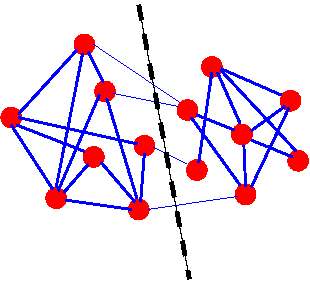
\includegraphics[width=0.3\linewidth]{figures/graphpartitioning.pdf}
    \caption{Partitioning of a graph using \textit{cuts} \parencite{fortunato-2009}.}
  \end{figure}

  These clusterings may be better or worse depending on the context, but a generally solid measure of ``clustering goodness'' is \textit{modularity} (\Cref{def:modularity}).

  \begin{definition}{Modularity}{modularity}
    For a given undirected graph $G = (V, E)$ and clustering $C$, let $$Q := \frac{1}{2m} \sum_{i=1}^{n} \sum_{j=1}^{n} \left(A_{ij} - \frac{d_i d_j}{2m}\right) \delta(s_i, s_j)\,,$$ with $\delta(\cdot, \cdot)$ the Kronecker delta indicating whether two vertices $v_i$ and $v_j$ belong to the same cluster \parencite{lambiotte-louvain-clustering}.
  \end{definition}

  Modularity is a measure of the quality of a clustering (also referred to as a partitioning) of $G$. It can also be written as the sum of individual cluster contributions
  $$Q = \sum_{c=1}^{n_C} Q_c = \frac{1}{2m} \sum_{c=1}^{n_C} \left[\sum_{v_i \in C_c} \sum_{v_j \in C_c} \left(A_{ij} - \frac{d_i d_j}{2m}\right)\right]\,,$$
  which might make its purpose a bit clearer.

  \section{Clustering Methods and Algorithms}
  In order to find ...
  Most clustering methods can be broadly categorised into spectral, partitional (such as k-means clustering), hierarchical, randomised, divisive and quality-optimisation algorithms.
  An interesting approach is Markov-Chain-Clustering, which may employ Simulated Annealing \cite{fortunato}.

  Community detection is, in principle, usually a ``very hard'' task given the vast number of possible system configurations as the graph grows in the number of edges or vertices, a statement which can be made more precise using complexity theory.
  In conventional complexity theory, problems are filed into different complexity classes when analysing their runtime and memory usage.
  There exist
  \begin{enumerate}[noitemsep,topsep=0pt,parsep=0pt,partopsep=0pt]
    \item NL (Nondeterministic Logarithmic space)
    \item P (Polynomial time)
    \item NP (Nondeterministic Polynomial time)
    \item PSPACE (Polynomial space)
    \item EXPTIME (Exponential time)
    \item EXPSPACE (Exponential space)
  \end{enumerate}
  computational complexity classes, sorted by the amount of problems contained in them (NL $\subseteq$ P $\subseteq$ NP $\subseteq$ PSPACE $\subseteq$ EXPTIME $\subseteq$ EXPSPACE).
  A particularly interesting open problem is whether P = NP, one of the millennium prize problems and the most important open problem in computer science.

  \begin{definition}{NP-Hardness}{np-hard}
    A problem is referred to as \textit{NP-hard} if and only if it is at least as hard as the hardest problems in the complexity class NP (nondeterministic polynomial time). Formally written,
    $$\mathrm{NP} := \bigcup_{k \in \N} \mathrm{NTIME}(n^k)$$
    the union of all decision problems with runtime bounded by $\mathcal{O}(n^k)$.
  \end{definition}

  Many community detection algorithms or problems relating to it are NP-hard \parencite{fortunato}.
  It is therefore often futile to employ exact algorithms as they quickly start to become infeasible for larger system sizes.

  Note that here we only consider an unweighted, undirected graph, while most clustering algorithms also allow working with a weighted graph $\tilde{G} = (V, \tilde{E})$ where $\tilde{E} \subset V \times V \times \R^+$ is a set of three-tuples $(v_i, v_j, w_{ij})$ instead of vertex pairs. Or equivalently, one can define a function $w: \tilde{E} \mapsto \R^+$ which maps vertex pairs (edges) to their respective weight.

  \subsection{Embeddings}
  Cosine-Similarity
  $$\rho_{ij} = \arccos\left(\frac{\vec{a_i} \vec{a_j}}{\norm{\vec{a_i}}_2 \cdot \norm{\vec{a_j}}}_2\right)$$

  \subsection{Girvan-Newman}
  The clustering method deduced in \cite{girvan-newman} was a clear revolution at the time and brought graph clustering / community detection methods closer to practicians.
  Optimises centrality and betweenness.

  \subsection{Louvain}
  The popular algorithm introduced by \cite{lambiotte-louvain-clustering} is based on modularity optimisation (cf. \Cref{def:modularity}) and has computational complexity of only $\mathcal{O}(m)$.
  It is referred to as the \textit{Louvain method} named after the University of Louvain in Belgium, alma mater of the first author.
  The Louvain method is divided into two phases: Phase One (local optimisation) and Phase Two (merging of vertices).
  \cite{grindrod-lecture-notes}.

  \begin{figure}[H]
    \centering
    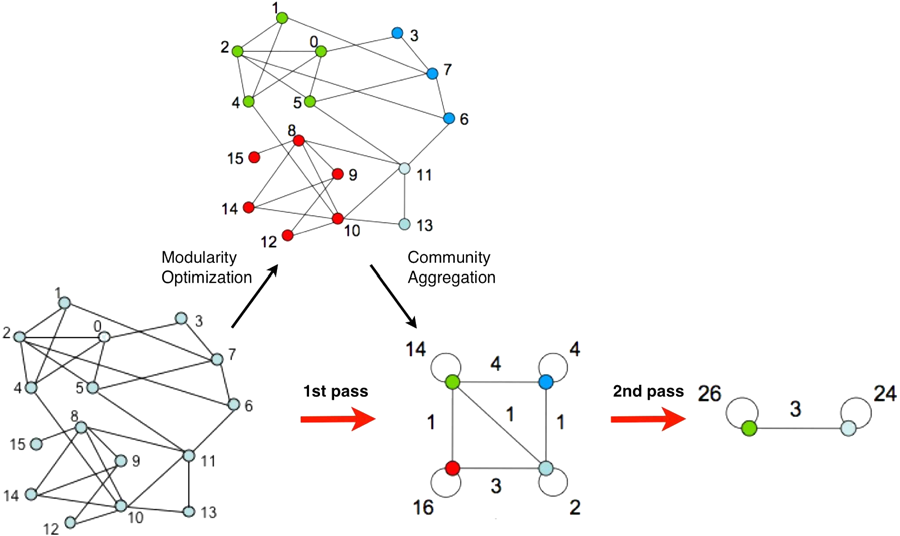
\includegraphics[width=\linewidth]{figures/blondel.png}
    \caption{Louvain Graph Clustering Method \cite{lambiotte-louvain-clustering}.}
  \end{figure}

  Louvain is very effective, in part because a change (improvement) in modularity obtained by reassigning an \textbf{isolated} (not yet clustered) vertex $v_i$ to a community $C_j$ may be explicitly obtained by
  \begin{equation}
    \Delta Q=\left[ \frac{\Sigma_{in}^{(j)} + k_{i,in}^{(j)}}{2 m} - \left(\frac{\Sigma_{tot}^{(j)} + k_{i}}{2m}\right)^2 \right] - \left[ \frac{\Sigma_{in}^{(j)}}{2m} - \left(\frac{\Sigma_{tot}^{(j)}}{2m}\right)^2 - \left(\frac{k_i}{2m}\right)^2 \right] \,,
    \label{eq:blondel-deltaQ}
  \end{equation}
  (as given in the original paper) which is highly useful from a computational perspective \parencite{lambiotte-louvain-clustering}.
  Here, we have $d_{i,in}^{(j)} := \left|\left\{(v_x, v_y) \in (C_j \times C_j) \cap E \;\big|\; v_x = v_i\right\}\right|$ the number of in-cluster edges connected to vertex $v_i$ and the corresponding $\Sigma_{in}^{(j)} := \sum_{v_i \in C_j} d_{i,in}^{(j)} = \left|(C_j \times C_j) \cap E\right|$ represents the total number of edges between vertices within the same cluster $C_j$ (so neglecting edges to vertices outside $C_j$).
  Likewise, $\Sigma_{tot}^{(j)} := \sum_{v_i \in C_j} d_i$ denotes the sum of vertex degrees within the cluster $C_j$ (so including contributions to outside nodes).

  In our case, the above weightings $k_j \in \R^+$ reduce to the degrees $d_j$ alone given that we operate on an unweighted, undirected graph $G = (V, E)$. Note that the above \Cref{eq:blondel-deltaQ} simplifies to
  \begin{equation}
    \Delta Q = \cancel{\frac{\Sigma_{in}^{(j)}}{2m}} + \frac{d_{i, in}^{(j)}}{2m} - \frac{\cancel{\left(\Sigma_{tot}^{(j)}\right)^2} + 2 \Sigma_{tot}^{(j)} d_i + \cancel{d_i^2}}{4m^2} - \cancel{\frac{\Sigma_{in}^{(j)}}{2m}} + \frac{\cancel{\left(\Sigma_{tot}^{(j)}\right)^2} + \cancel{d_i^2}}{4m^2} = \frac{d_{i, in}^{(j)}}{2m} - \frac{\Sigma_{tot}^{(j)} d_i}{2m^2} \,.
    \label{eq:blondel-deltaQ-simplified}
  \end{equation}

  In more general terms, one may obtain the impact of moving a vertex $v_i \in V$ from cluster $C_a$ to $C_b$ by considering their individual contributions
  $$Q_c = \sum_{v_i \in C_c} \sum_{v_j \in C_c} \left(A_{ij} - \frac{d_i d_j}{2m}\right) = \frac{\Sigma_{in}^{(j)}}{2m} - \left(\frac{\Sigma_{tot}^{(j)}}{2m}\right)^2\,,$$
  to the total modularity $Q = \sum_{c=1}^{n_C} Q_c^{(c)}$, which are
  \begin{align*}
    \tilde{Q}_c^{(a)} & = \frac{\Sigma_{in}^{(a)} - d_{i, in}^{(a)}}{2m} - \left(\frac{\Sigma_{tot}^{(a)} - d_i}{2m}\right)^2\,, \\
    \tilde{Q}_c^{(b)} & = \frac{\Sigma_{in}^{(b)} + d_{i, in}^{(b)}}{2m} - \left(\frac{\Sigma_{tot}^{(b)} + d_i}{2m}\right)^2\,,
  \end{align*}
  after moving vertex $v_i$ from cluster $C_a$ to $C_b$.
  So the change in individual cluster modularity is given by the terms
  \begin{align*}
    \Delta Q_c^{(a)} & = \tilde{Q}_c^{(a)} - Q_c^{(a)} = \frac{-d_{i, in}^{(a)}}{2m} - \frac{d_i^2 - 2 \Sigma_{tot}^{(a)} d_i}{4m^2}\,, \\
    \Delta Q_c^{(b)} & = \tilde{Q}_c^{(b)} - Q_c^{(b)} = \frac{d_{i, in}^{(b)}}{2m} - \frac{d_i^2 + 2 \Sigma_{tot}^{(b)} d_i}{4m^2}\,,
  \end{align*}
  which yield the total modularity change $\Delta Q = \Delta Q_c^{(a)} + \Delta Q_c^{(b)}$ in the general case.
  Considering the special case when vertex $v_i \in V$ is still isolated, so when $C_a = \{v_i\}$ contains exactly that one vertex, we can further simplify to
  $$\Delta Q = \cancel{\frac{d_i^2}{4m^2}} + \frac{d_{i,in}^{(b)}}{2m} - \frac{\cancel{d_i^2} + 2 d_i \Sigma_{tot}^{(b)}}{4m^2} = \frac{d_{i,in}^{(b)}}{2m} - \frac{\Sigma_{tot}^{(b)} d_i}{2m^2} \,,$$
  because $\Sigma_{in}^{(a)} = 0$, $\Sigma_{tot}^{(a)} = d_i$ and therefore $\Delta Q_c^{(a)} = \frac{d_i^2}{4m^2}$, and we arrive at the same expression given by \cite{lambiotte-louvain-clustering} (\Cref{eq:blondel-deltaQ-simplified}), for the special case when $C_a = \{v_i\}$.
  Note that the modularity contribution $Q_c = 0$ for an empty cluster.

  This modularity gain of course is not restricted to the Louvain method in and of itself, it applies to all clustering methods and is relevant to those that operate on modularity.

  Louvain is among the most widely used techniques for graph clustering and is available in numerous software packages.

  % https://en.wikipedia.org/wiki/Louvain_method

  \subsection{Chinese Whispers}
  This method, like the Louvain method, also initialises the algorithm by assigning each vertex its own category (cluster).

  \begin{algorithm}[language=pseudo, caption={\centering The \textit{Chinese Whispers} algorithm due to \cite{cw-biemann}}]
Input: an undirected graph $G = (V, E)$.
Output: a graph clustering $C = \{C_i\}_{i=1, ..., n_C}$ into $n_C$ classes.

Initialise with $n_C = n$ classes, one per vertex.
while there are changes, do
  for $v_i$ in shuffle($V$), do
    Set $s_i = 3$
  end
end
  \end{algorithm}

  Corresponds to an agent-based simulation of a social network \cite{cw-biemann}.
  Similar to Markov-Chain-Clustering \cite{van-dongen}, \cite{fortunato}.

  The algorithm may equivalently be defined by considering the \textit{class matrix} $\mathcal{D} \in \{0, 1\}^{n \times n_C}$ of a graph $G = (V, E)$ in which rows represent nodes and columns represent clusters $C_j \in C$.
  So $G_{ij} = 1$ if $v_i$ belongs to $C_j$ and $0$ otherwise.
  The algorithm operates iteratively and updates the class matrix $\mathcal{D}^{(k)}$ using
  $$M: \{0, 1\}^{n \times n_C} \mapsto \{0, 1\}^{n \times n_C}, \quad \{M(\mathcal{D})\}_{ij} = \mathcal{D}_{ij}$$ % TODO: this is not great
  $$\mathcal{D}^{(k+1)} = M(\mathcal{D}^{(k)}) A, \quad k = 0, 1, 2, ..., N$$
  per iteration $k$, where $\mathcal{D}^{(0)} = I$ is the identity, corresponding to the initialisation of individual classes for each vertex.

  The paper also discusses acquisition of word classes (semantic fields), where they ran Chinese Whispers against the British National Corpus (BNC) to identify clusters of similar words.
  In order to improve performance, they cut off the 2000 most frequent words in the corpus which we will also employ.
  This set of highly frequent words is likely to contain the \textit{core vocabulary} of the language including, but not limited to, pronouns, conjunctions, prepositions and similar parts of speech.
  \cite{cw-biemann} identified 282 clusters, 26 of which contained more than 100 words.
  Word clustering methods such as this one may even be used to improve part-of-speech tagging \parencite{ushioda-improved-pos-tagging}.

  \begin{table}[H]
    \centering
    \caption{Table ordered by size \cite{cw-biemann}.}
    \begin{tblr}{colspec={ X[c] X[4,j,m] }}
      \hline
      Size $|C_i|$ & Sample Words                                                                            \\
      \hline
      18432        & secret, officials, transport, unemployment, farm, county, wood, procedure, grounds, ... \\
      4916         & busy, grey, tiny, thin, sufficient, attractive, vital, ...                              \\
      4192         & filled, revealed, experienced, learned, pushed, occurred, ...                           \\
      3515         & White, Green, Jones, Hill, Brown, Lee, Lewis, Young, ...                                \\
      2211         & Ian, Alan, Martin, Tony, Prince, Chris, Brian, Harry, Andrew, Christ, Steve, ...        \\
      1855         & Central, Leeds, Manchester, Australia, Yorkshire, Belfast, Glasgow, Middlesbrough, ...  \\
    \end{tblr}
  \end{table}

  \subsection{Watset}
  A more recent work \cite{watset} describes a meta-algorithm for graph clustering in the context of Natural Language Processing, which can be based on Chinese Whispers and also other methods.

  \subsection{Spectral Clustering Methods}
  % very good resource: https://theory.epfl.ch/vishnoi/Lxb-Web.pdf
  \cite{fortunato}.

  \subsection{Fiedler}
  \cite{fortunato}.

  \section{Method}
  We shall also remove the 2000 most frequent words

  \section{Results}
  An itemize with some semantic field clusters we found

  \begin{table}
    \centering
    \caption{Results ordered by size.}
    \begin{tblr}{colspec={ X[c] X[4,j,m] }}
      \hline
      Size $|C_i|$ & Sample Words                                                                            \\
      \hline
      18432        & secret, officials, transport, unemployment, farm, county, wood, procedure, grounds, ... \\
    \end{tblr}
  \end{table}

  Plotty plot

  Apply to Karate Club

  Computational complexity table from \cite{watset}, also referencing complexity section above. Fortunato also has complexities.

  \section{Author analysis?}
  Authors whose works circulate around these semantic fields:
  bla bla, maybe not that interesting

  \pagebreak
  \section{Discussion and Outlook}
  Bla

  \pagebreak
  \printbibliography

  \appendix
  \section{Appendix Things?}
\end{document}
